% !TeX root = ../main.tex
\section{Kết quả thực nghiệm}
\subsection{Cách đánh giá}
\begin{itemize}
\item \textbf{Chuẩn hóa:} NFKC, chuyển chữ thường, gộp khoảng trắng; bỏ
\texttt{\#\#LTLine\#\#}, \texttt{\#\#LTFigure\#\#} ở GT và dự đoán.
\item \textbf{Chỉ số:} CER/WER dựa trên số phép thay thế, xóa, chèn. Precision
(P) là tỷ lệ token dự đoán khớp GT; Recall (R) là tỷ lệ token GT được nhận ra;
F1 kết hợp P và R. Token tách theo khoảng trắng, đếm số lần xuất hiện, không xét
thứ tự khi tính P/R/F1.
\item \textbf{Tổng hợp:} tính điểm từng ảnh rồi lấy trung bình đều. Thời gian xử
lý không tính tải mô hình/dữ liệu, chấm điểm hay ghi kết quả. CER/WER càng thấp
càng tốt; P/R/F1 càng cao càng tốt.
\end{itemize}

\subsection{Kết quả chung trên 8.999 ảnh}
Các tỷ lệ trong bảng dùng \%; thời gian dùng giây/ảnh.

\begingroup\fontsize{10}{11.5}\selectfont
\setlength{\tabcolsep}{4pt}
\begin{tabular*}{\linewidth}{@{\extracolsep{\fill}}lrrrrrr@{}}
\toprule
\textbf{Mô hình} & \textbf{CER}$\downarrow$ & \textbf{WER}$\downarrow$ &
\textbf{P}$\uparrow$ & \textbf{R}$\uparrow$ & \textbf{F1}$\uparrow$ & \textbf{Giây/ảnh}$\downarrow$ \\
\midrule
Florence & 61,27 & 79,33 & 53,41 & 31,69 & 38,55 & 5,597 \\
EasyOCR & 57,60 & 82,42 & 43,86 & 31,96 & 36,51 & 1,363 \\
docTR & 47,86 & 62,89 & 78,79 & 68,86 & 72,76 & 0,601 \\
PaddleOCR & \textbf{33,97} & \textbf{43,25} & \textbf{85,17} & \textbf{72,97} & \textbf{77,75} & \textbf{0,403} \\
Tesseract & 47,94 & 66,65 & 59,73 & 41,13 & 47,84 & 0,906 \\
\bottomrule
\end{tabular*}

\par\endgroup
\begin{itemize}
\item \textbf{PaddleOCR:} CER/WER thấp nhất, F1 cao nhất (77,75\%), hơn docTR 4,99 điểm.
\item \textbf{Florence:} F1 38,55\%; 1.586 đầu ra có cờ có thể bị cắt ở 1.024 token.
\end{itemize}

\clearpage
\subsection{Ảnh hưởng của vị trí và loại che khuất}
\begingroup\fontsize{10}{11.5}\selectfont
\setlength{\tabcolsep}{4pt}
\begin{tabular*}{\linewidth}{@{\extracolsep{\fill}}lrrrrrr@{}}
\toprule
& \multicolumn{3}{c}{\textbf{Che vùng chữ: 6.000 ảnh}} &
\multicolumn{3}{c}{\textbf{Che vùng phi văn bản: 2.999 ảnh}} \\
\cmidrule(lr){2-4}\cmidrule(lr){5-7}
\textbf{Mô hình} & CER & WER & F1 & CER & WER & F1 \\
\midrule
Florence & 56,03 & 77,58 & 38,69 & 71,74 & 82,83 & 38,27 \\
EasyOCR & 55,40 & 81,05 & 36,75 & 62,00 & 85,18 & 36,04 \\
docTR & 43,85 & 59,77 & 71,12 & 55,87 & 69,14 & 76,02 \\
PaddleOCR & 24,68 & 38,12 & 76,76 & 52,55 & 53,51 & 79,73 \\
Tesseract & 43,78 & 63,74 & 49,05 & 56,26 & 72,48 & 45,41 \\
\bottomrule
\end{tabular*}

\par\endgroup
PaddleOCR dẫn đầu cả hai nhóm. F1 ở nontext cao hơn text 2,97 và 4,90 điểm với
PaddleOCR và docTR, dù WER cao hơn. F1 không xét thứ tự token, còn WER có xét. Các nhóm
khác nhau về trang, nên đây là so sánh mô tả theo vị trí che.

\noindent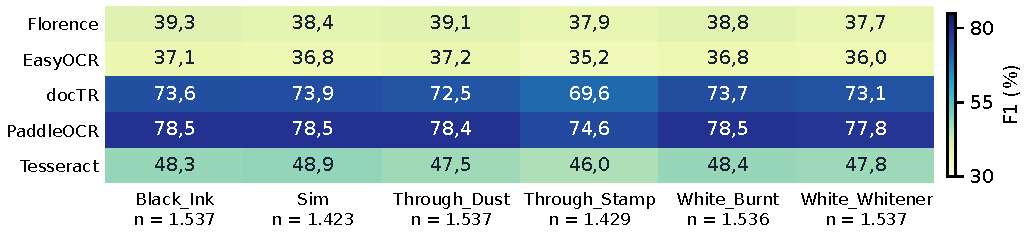
\includegraphics[width=\linewidth]{img/robustness.pdf}
{\footnotesize Hình 1. F1 theo sáu loại che khuất trên cùng tập 8.999 ảnh;
$n$ là số ảnh hợp lệ của mỗi loại.\par}
PaddleOCR có F1 cao nhất ở cả sáu loại. Through\_Stamp có F1 thấp nhất ở bốn
OCR; PaddleOCR đạt 74,58\%, thấp hơn 3,94 điểm so với Black\_Ink. Florence có
F1 thấp nhất ở White\_Whitener (37,74\%).

\subsection{Ví dụ đọc đúng và đọc sai}
Đoạn trích từ kết quả đã lưu; mã bài/trang và điểm của cả ảnh sau chuẩn hóa:

{\fontsize{10}{11.3}\selectfont
\begin{itemize}
\item \textbf{PaddleOCR -- Black\_Ink 1\%, mã 1601.04736/36:}
GT và dự đoán đều có ``Simulation Results for Parameters in FitzHugh-Nagamu Model''.
CER = WER = 0\%: toàn bộ văn bản dự đoán khớp tham chiếu sau chuẩn hóa.
\item \textbf{Tesseract -- Through\_Dust 1\%, mã 1507.03120/23:}
GT ``Mod.'' và ``24'' thành ``Mod,'' và ``os''; CER 1,63\%, WER 6,90\%.
Ví dụ cho thấy lỗi dấu câu và nhầm chữ--số.
\item \textbf{Florence -- White\_Burnt 2\%, mã 1408.3064/10:}
GT ``WIENER-WINTNER'' thành ``WIENER-WINNER''; WER 55,77\%.
Đầu ra có chuỗi số/ký hiệu dài và đạt 1.024 token: vừa có từ nhận sai vừa có cờ
có thể bị cắt.
\end{itemize}}

\subsection{Hiệu quả và giới hạn}
\begin{itemize}
\item \textbf{Chất lượng và chi phí:} PaddleOCR dùng 11,89 MiB và 0,403 giây/ảnh;
docTR dùng 24,24 MiB và 0,601 giây/ảnh trên T4, với F1 thấp hơn 4,99 điểm.
\item \textbf{Phương án CPU:} Tesseract có tệp 3,92 MiB, F1 47,84\%.
Thời gian CPU/GPU không phải phép đo trên cùng phần cứng.
\item \textbf{Giới hạn:} GT ngắn có thể làm CER/WER vượt 100\%; giữ nguyên các giá trị này.
\end{itemize}
